
\chapter{Elliptische Kurven}

\section{Allgemeine Funktionsweise} \label{ECC_DLP}

In klassischen Methoden asymmetrischer Verschlüsselungen wie Diffie-Hellman und ElGamal basiert die
Verschlüsselung auf endlichen, arithmetischen Feldern modulo einer großen Primzahl $p$ oder $p^n$.
Dabei werden die Vorteile und die Falltür-Funktionalität des diskreten Logarithmus-Problem genutzt.
(siehe Kapitel: \ref{DLP} \nameref{DLP})

Im Kontext der Verschlüsselung mittels elliptischer Kurven wird eine algebraische Gruppe über Punkte
auf einer elliptischen Kurve definiert. 
Die elliptische Kurve erfüllt die folgende Kurvengleichung:

\begin{center}
$y^2 = x^3 + a*x + b$
\end{center}

Dabei sind die Koeffizienten $a$ und $b$ fest definiert.
Eine Kurve mit den Koeffizienten $a = -1$ und $b = 0$ ergibt folgende elliptische Kurve:

\begin{figure}[H]
	\begin{center}
		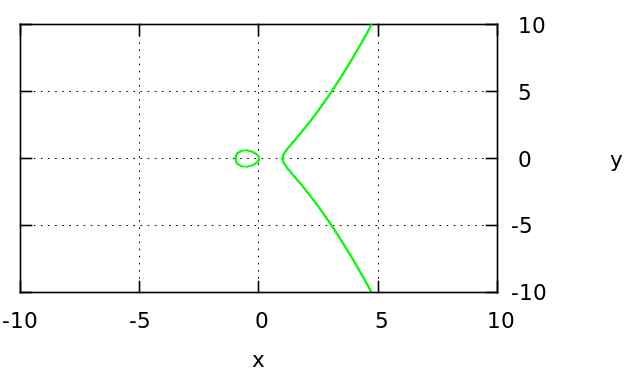
\includegraphics[keepaspectratio=true, scale=0.4]{./pictures/example_curve_1a.png}
	\end{center}
	\caption{$y^2 = x^3 -x$}\label{example_1}
\end{figure}

Eine Kurve mit $a = 1$ und $b = 1$ ergibt folgende elliptische Kurve:

\begin{figure}[H]
	\begin{center}
		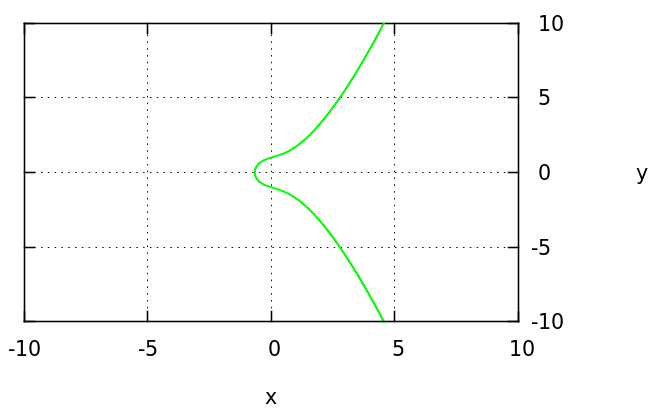
\includegraphics[keepaspectratio=true, scale=0.4]{./pictures/example_curve_2a.png}
	\end{center}
	\caption{$y^2 = x^3 +x +1$}\label{example_2}
\end{figure}

Eine elliptische Kurve ist demnach definiert über die zwei kurven-lokale Konstanten $a$ und $b$.
Die Schreibweise zur Definition einer elliptischen Kurve ist $E(a;b)$.
Punkte auf der elliptischen Kurve sind definiert über ihre $x$ und $y$-Koordinaten. Also: $p = (x;y)$.

Um eine algebraische Gruppe über Punkten einer elliptischen Kurve definieren zu können, muss die additive
Operation auf Elementen der Gruppe definiert werden und ein neutrales Element existieren.

Für jede elliptische Kurve gilt, dass jede Gerade, definiert durch zwei Punkte der Kurve, immer genau einen
dritten Schnittpunkt mit der elliptischen Kurve besitzt.

Seien nun $P$ und $Q$ Punkte auf einer elliptischen Kurve, so existiert ein Schnittpunkt der Geraden durch $P$
und $Q$ mit einem weiteren Punkt $R$ der Kurve. Wenn $P = Q$, ist die Gerade definiert als die Tangente am
Punkt $P$. Da es exakt drei Schnittpunkte einer so definierten Gerade mit der elliptischen Kurve gibt, 
ist die Existenz und Einzigartigkeit von $R$ garantiert.

Der Punkt $O$ sei ein weiterer Punkt, welcher die elliptische Kurvengleichung erfüllt. Er gilt als das neutrale
Element und ist per Konvention ein Punkt im Unendlichen.

Betrachtet man nun eine Gerade zwischen $R$ und $O$, so schneidet diese einen dritten Punkt der Kurve. 
Dieser ist definiert als $P + Q$.

Sei $OO$ der Schnittpunkt der Tangente an $O$ mit der Kurve, wird der Schnittpunkt der Geraden zwischen $OO$ und $P$ mit der elliptischen Kurve nun $-P$ genannt.\cite{explicit_addition}

Die folgenden Gleichungen belegen die genannten Berechnungen:
	
\begin{center}
	$P + Q = Q + P$
	
	$P + O = P$
	
	$(-P) + P = O$
\end{center}

Zusammengefasst gelten folgende Definitionen für Operationen auf der Gruppe definiert durch Punkte auf der 
elliptischen Kurve:

\textit{\textbf{Negation:}}

Die Negation eines Punktes auf einer Kurve ist definiert über die Negation der $y$-Komponente des Punktes.
Also: $P = (x;y)$ und: $-P = (x;-y)$.

\textit{\textbf{Addition:}}

Eine Addition zweier Punkte $P$ und $Q$ auf einer Kurve ist definiert, indem eine Gerade zwischen $P$ und $Q$ 
gezogen wird. Der dritte Schnittpunkt der Geraden mit der Kurve (erster Schnittpunkt auf $P$, zweiter 
Schnittpunkt auf $Q$) wird nun negiert. Der nun errechnete Punkte bildet das Ergebnis der Addition.

\textit{\textbf{Punkt verdoppeln:}}

Ein Punkt $P$ auf der Kurve wird verdoppelt, indem die Tangente an $P$ mit der Kurve geschnitten wird. Der Schnittpunkt
ist nun $-(P+P)$.

\textit{\textbf{Multiplikation:}}

Mit den aktuell definierten Operationen auf elliptischen Kurven entsteht eine Gruppe. 
Eine multiplikative Operation ist nicht definiert und auch nicht trivial zu konstruieren.
Im weiteren Verlauf wird jedoch eine Multiplikation benötigt um einen asynchronen Schlüsselaustausch zu ermöglichen.

Da ausschließlich multiplikative Operationen eines Punktes mit einem Integer erforderlich sind, wird 
eine Multiplikation im Folgenden durch eine wiederholte Addition eines Punktes simuliert.
Eine Multiplikation zweier Punkte ist weiterhin nicht definiert.
\newline
\newline
Finite elliptische Kurven können über $\mathbb{Z}_p$ oder $GF(p^n)$ mit $p$ als Primzahl definiert werden.
Im Kontext der Kryptografie werden jedoch meist nur Kurven über $\mathbb{Z}_p$ und $GF(2^n)$ genutzt.
Der Einfachbarkeitshalber sind alle Beispiele über $\mathbb{Z}_p$ definiert.


\section{Asynchroner Schlüsseltausch}

Asynchroner Schlüsseltausch wird gemeinhin genutzt um einen Schlüssel für eine weitere synchrone Verschlüsselung über 
einen unsicheren Kanal zu transportieren. Die bekannten Algorithmen und Schemata wie Diffie-Hellman stützen direkt auf
das diskrete Logarithmus-Problem. Die gleichen Prinzipien können jedoch auch mit Hilfe elliptischer Kurven erreicht 
werden. Dabei handelt es sich um analoge Verfahren zu ebendiesen und nicht um die exakten.

Im Weiteren werden beide Teilnehmer zwischen denen ein Schlüsselaustausch stattfinden soll mit \textit{Alice} und \textit{Bob}
referenziert.

Die folgenden Attribute gelten für alle vorzustellenden Algorithmen:

Als $E$ wird die elliptische Kurve bezeichnet aus $GF(q)$ wobei $q = p^n$ eine bevorzugt große Zahl darstellt. 
Die Kurvenparameter der genutzten Kurve sind öffentlich.
Weiterhin muss eine eindeutige, öffentlich zugängliche Funktion existieren, welche eine Nachricht $m$ auf einen Punkt $P_m$ der 
elliptischen Kurve abbildet: $f:m \rightarrow P_m$.

\subsection{Diffie-Hellman}

Ein analoger Algorithmus zu Diffie-Hellman, basieren auf elliptischen Kurven geht folgenderweise vor.

Öffentlich bekannt ist ein gemeinsamer Punkt $G$ (erzeugendes Element der Gruppe) auf der elliptischen Kurve $E$.
Beide Teilnehmer des Schlüsselaustausches erstellen ihr jeweiliges Schlüsselpaar bestehend aus einem privaten Schlüssel
$d$ mit $0 < d < N$ und $ggt(d, N) = 1$\footnote{Größter gemeinsamer Teiler (auch gcd)} mit $N = |E|$ und einem öffentlichen 
Schlüssel $Q$ mit $Q = d * G$.

Alice' Schlüsselpaar: $(d_A, Q_A)$

Bobs Schlüsselpaar: $(d_A, Q_A)$

Der öffentliche Part des Schlüsselpaares ist jeweils beiden Kommunikationsteilnehmern bekannt.
Alice berechnet nun $d_A*Q_B = (x_k, y_k)$. Bob berechnet $d_B*Q_A = (x_k, y_k)$.
Die X-Koordinate $x_k$ des Ergebnispunktes auf der elliptischen Kurve ist nun das gemeinsame Geheimnis, welches
ausschließlich Alice und Bob bekannt ist.

Die Gültigkeit, dass beide Teilnehmer das gleiche Ergebnis berechnen zeigt sich durch folgende Gleichungsauflösung 
$d_A*Q_B = d_A*d_B*G = d_B*d_A*G = d_B*Q_A$.

Um aus dem gemeinsamen Geheimnis einen Schlüssel zu erzeugen, wird die X-Koordinate des Ergebnispunktes meist kryptografisch gehashed und
als symmetrischer Schlüssel verwendet.

\subsection{Massey-Omura}

Das Schema von Massey-Omura ist ein von Diffie-Hellman motivierter Algorithmus für den asynchronen Schlüsseltausch.

Die Vorgehensweise ist wie folgt. Alice generiert sich einen geheimen Wert $c$ mit $0 < c < N$ und $ggt(c,N) = 1$.
Alice überträgt nun die Nachricht $c * P_m$ an Bob.
Bob generiert sich einen geheimen Wert $d$ mit $0 < d < N$ und $ggt(d,N) = 1$ und überträgt die Nachricht
$d * (c * P_m)$ an Alice.
Alice antwortet Bob mit der Nachricht $c' * (d * c * P_m) = d * P_m$ wobei gilt, dass $(c * c') = 1\ mod\ N$.
Bob berechnet nun $d' * d * P_m = P_m$ und erhält die ursprüngliche Nachricht $P_m$. Auch hier gilt, dass $(d * d') = 1\ mod\ N$.

\subsection{ElGamal}

Auch eine Variation vom klassischen ElGamal kann mit elliptischen Kurven genutzt werden.
Öffentlich bekannt ist, wie bei Diffie-Hellman, ein gemeinsamer Punkt $G$ (erzeugendes Element der Gruppe) auf der elliptischen Kurve $E$.

Bob generiert sich einen geheimen Wert $d$ und veröffentlicht den Punkt auf der Kurve $d * G$.
Alice generiert sich einen Wert $c$ und sendet Bob das Tupel $(c * G, P_m + c*(d*G))$. 
Bob kann nun den ersten Teil des übertragenen Tupels mit seinem geheimen Wert $d$ multiplizieren und vom zweiten Teil des Tupels abziehen.
Das Ergebnis der Subtraktion ist die eigentliche zu geheime Nachricht $P_m$.

Die Auflösung lässt sich zeigen durch: $(P_m + c * (d * G)) - (d * (c * G)) = P_m$.

\section{Komplexität und Berechenbarkeit von ECC}

Wie in den vorherigen Kapiteln (siehe Kapitel: \ref{ECC_DLP} \nameref{ECC_DLP}) erwähnt und erläutert, basiert die Komplexität
von Kryptografie über elliptische Kurven auf dem diskreten Logarithmus-Problem für ebendiese 
(ECDLP\footnote{elliptic-curve discrete logarithm problem}).
Zum aktuellen Zeitpunkt sind noch keine Algorithmen bekannt, welche dieses Problem effizient oder in subexponentieller Zeit
lösen.
Die effizientesten derzeit bekannten Algorithmen basieren auf dem Pollard-$\rho$ und dem Pollard-$\lambda$-Methoden\cite{ecc_complexity}.

Die Pollard-$\rho$-Methode benötigt etwa $\sqrt{\pi * n / 2}$ Schritte, die Pollard-$\lambda$-Methode etwa $2*\sqrt{n}$ Schritte.
Ein Schritt entspricht grob einer eigenständigen Gruppenoperation auf der elliptischen Kurve. Beide Methoden eignen sich
sehr gut zum Parallelisieren. Verschiedene Forschungen haben ergeben, dass beide Pollard-Methoden um kleinere Faktoren
schneller umgesetzt werden können\cite{ecc_complexity}.

Die nachfolgende Tabelle stellt die Komplexität des Lösens des ECDLP für elliptische Kurven als benötigte Zeit zum Berechnen
des diskreten Logarithmus-Problem dar, abhängig der jeweiligen Schlüssellänge.

\begin{center}
	\begin{tabular}{ |c|c|c| }
		\hline
		Schlüssellänge in bits & Pollard-$\rho$ & MIPS years\footnote{1 Jahr mit 1.000.000 Instruktionen/Sekunde} \\
		\hline
		\hline
		160 & $2^{80}$ & $8.5 * 10^{11}$ \\
		\hline
		192 & $2^{96}$ & $5.6 * 10^{16}$ \\
		\hline
		224 & $2^{112}$ & $3.7 * 10^{21}$ \\
		\hline
		256 & $2^{128}$ & $2.4 * 10^{26}$ \\
		\hline
		384 & $2^{192}$ & $4.4 * 10^{45}$ \\
		\hline
		521 & $2^{260}$ & $1.3 * 10^{66}$ \\
		\hline
	\end{tabular}
\end{center}

\newpage

\section{Unsichere Kurven}

Die Forschung, welche elliptischen Kurven möglicherweise Unsicherheiten beinhalten oder besonders anfällig für bestimmte
Angriffe sind, ist hochaktuell. Jedoch steht fest, dass es Unterschiede bezüglich der Sicherheit von elliptischen Kurven
gibt, abhängig ihrer Kurvenparameter. Drei mögliche Klassen von Kurvenparametern/Kurven, welche zu schwächeren Kurven
führt werden im Folgenden behandelt und erläutert.

In die erste Klasse an angreifbaren elliptischen Kurven fallen Kurven $E$ über $\mathbb{F}_q$ mit einem $n$, welches 
$q^B -1$ teilt. Für kleine $B$ sind die Kurven angreifbar, wie von Menezes, Okamoto und Vanstone beschrieben\cite{ecc_attack1}.
Der Angriff reduziert das ECDLP auf das klassische, traditionelle diskrete Logarithmus-Problem in eine Teilgruppe von $\mathbb{F}_q$.

Eine zweite angreifbare Klasse elliptischer Kurven sind Kurven $E$ über $\mathbb{F}_q$ mit $\#E(\mathbb{F}_q) = q$.
Semaev\cite{ecc_attack2}, Smart\cite{ecc_attack2b}, Satoh and Araki\cite{ecc_attack2b} beschreiben einen Angriff auf Kurven dieser Art. Dabei kann die Gruppe der elliptischen
Kurve effizient auf eine additive Gruppe von $\mathbb{F}_q$ abgebildet werden.

Die dritte Klasse beschreibt Kurven definiert über $\mathbb{F}_q$ mit $q = 2^m$ und einem zusammengesetzten $m$.
Die Angriffe erfolgen über sogenanntes "Weil-Descent"\cite{ecc_attack3}. Sie sind noch immer Gegenstand aktueller Forschungen.

Generell sind Kurven für die praktische oder theoretische Angriffsmöglichkeiten existieren, zu meiden.

\newpage

\section{Gegenüberstellung von Schlüssellängen}

Im Folgenden werden die Schlüssellängen verschiedener synchroner und asynchroner kryptografischer Algorithmen
bezüglich ihrer Sicherheitsbits miteinander verglichen.\cite{security_bits}
Wie klar zu erkennen ist, benötigt eine Verschlüsselung/Schlüsselübergabe für eine gleiche Anzahl an Sicherheitsbits
deutlich kürzere Schlüssel. Damit einher gehend kann eine Berechnung mit elliptischen Kurven deutlich schneller von Statten gehen,
als beispielsweise RSA oder Diffie-Hellman basieren auf dem diskreten Logarithmus-Problem.

\begin{center}
	\begin{tabular}{ |p{2.5cm}|p{2.5cm}|p{2.5cm}|p{2.5cm}|p{2.5cm}| }
		\hline
		Sicherheitsbits & Symmetrische \newline Algorithmen & FFC\footnote{finite field cryptography} \newline zB. DSA, D-H  &  IFC\footnote{integer-factorization cryptography} \newline zB. RSA & ECC\footnote{elliptic curve cryptography} \newline zB. ECDSA\\
		\hline
		\hline
		80 & 2TDEA    & $L = 1024$ \newline $N = 160$  & $k = 1024$  & $f = 160-223$ \\
		\hline
		112 & 3TDEA   & $L = 2048$ \newline $N = 224$  & $k = 2048$  & $f = 224-255$ \\
		\hline
		128 & AES-128 & $L = 3072$ \newline $N = 256$  & $k = 3072$  & $f = 256-283$ \\
		\hline
		192 & AES-192 & $L = 7680$ \newline $N = 384$  & $k = 7680$  & $f = 284-511$ \\
		\hline
		256 & AES-256 & $L = 15360$ \newline $N = 512$ & $k = 15360$ & $f = 512+$ \\
		\hline
	\end{tabular}
\end{center}

\iffalse 

	Plot erstellen mit gnuplot:
	
	set view 0,0
	set isosample 500,500
	set contour base
	set cntrparam levels discrete 0
	unset surface
	set grid
	unset key
	unset ztics
	set xlabel 'x'
	set ylabel 'y'
	f(x,y) = x**3 + 3*x + 2 - y**2
	splot [-10:10][-10:10] f(x,y)

\fi